\documentclass[aspectratio=169]{beamer}
\usetheme{metropolis}
\usepackage{multicol}
\usepackage{scrextend}
\usepackage{amsmath}
\usepackage{tikz-cd}
\newenvironment{mb}[1]{\begin{block}{#1}\vspace{.05cm}\begin{addmargin}[3ex]{0em}}{\end{addmargin}\end{block}}
\linespread{0.9}
\makeatletter
\g@addto@macro\normalsize{%
\setlength{\abovedisplayskip}{.7pt}
\setlength{\belowdisplayskip}{.7pt}
\setlength{\abovedisplayshortskip}{.7pt}
\setlength{\belowdisplayshortskip}{.7pt}
}
\makeatother
\setlength{\parindent}{0cm}
\setlength{\parskip}{.3cm}
\title{Differential Geometry and Lie Group Theory}
\date{\today}
\author{Sayako Hoshimiya (Yutong "Hypatia" Zhang)}
\institute{Beijing LGBT Center}
\begin{document}
\maketitle
\begin{frame}{Review of Algebra - Vector Space}
\vspace{.5cm}
\begin{figure}[]
\centering
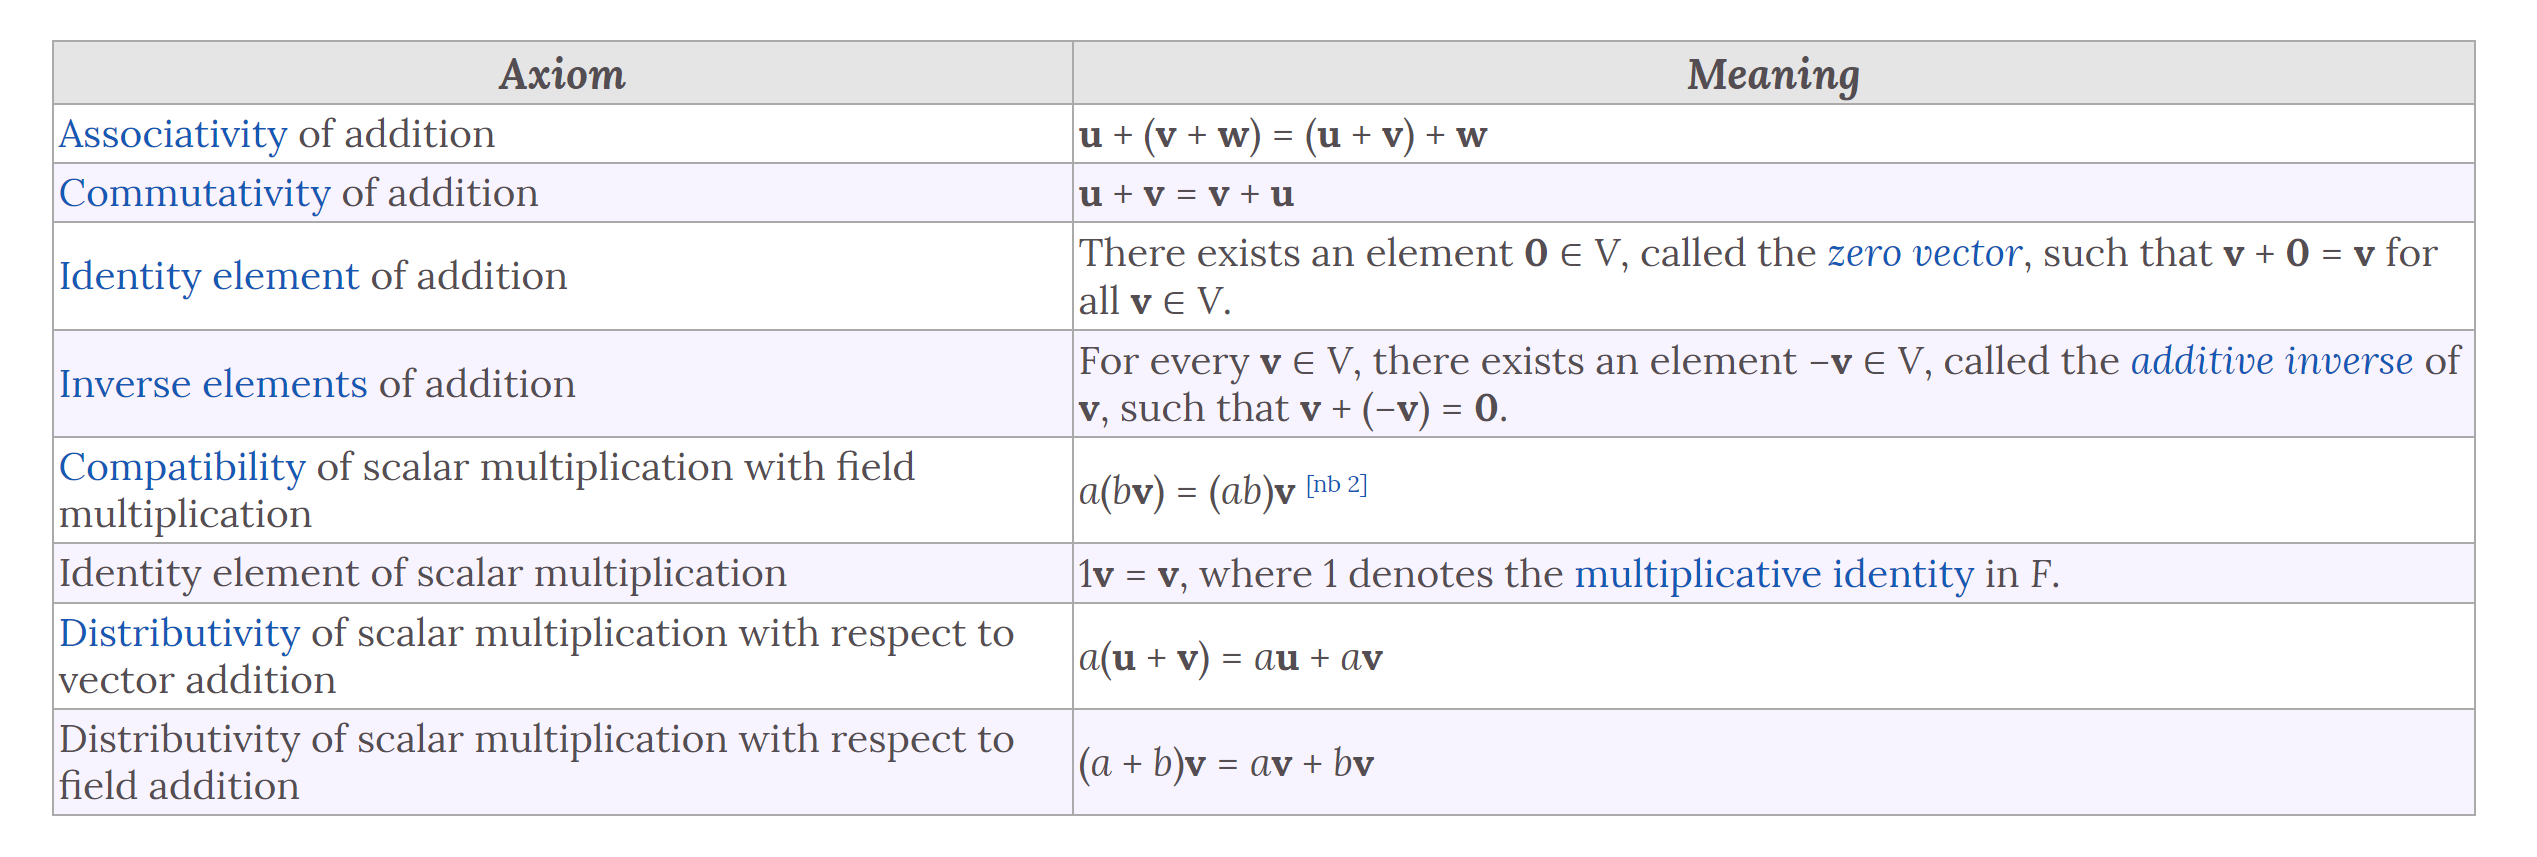
\includegraphics[width=\textwidth]{vectorspaceaxioms}
\caption{Vector Space Axioms}
\end{figure}
\end{frame}
\begin{frame}{Review of Algebra - Change of Bases}
\begin{columns}
\begin{column}{0.5\textwidth}
Conventionally in modern geometry, \alert{matrices} are denoted with a superscript and a subscript, e.g. $A^i_j$ with the superscript the row and the subscript the column. When we write change of basis matrix, we use right multiplication with column vector, e.g. ${v'}^i[e'_i]=\sum_{i=1}^nA^i_jv^j[e_j]$
\\~\\
Note that if we write the basis in row vector and left multiply it with a matrix, then the inverse of this matrix is the coordinate transformation matrix when used with the manner described above.
\end{column}
\begin{column}{0.5\textwidth}
A \alert{permutation} of ordered tuple is a autobijection, i.e. a one-to-one onto map from itself to itself. The permutations of an $n$-element set is denoted as $S_n$. For a permutation $\sigma$, the \alert{parity} $\operatorname{sgn}\sigma$ is defined as the number of transpositions in its decomposition.
\\~\\
For an $n\times n$ matrix $A$, the determinant is defined as $$\det A=\sum_{\sigma\in S_n}(\operatorname{sgn}\sigma)\prod_{i=1}^nA^i_{\sigma(i)}$$
\end{column}
\end{columns}
\end{frame}
\begin{frame}{*Review of Algebra - Covariance \& Contravariance}
Continuing the discussion from the previous slide on the left bottom part, we notice that we have
\\~\\
\vspace{.3cm}
\begin{columns}
\begin{column}{0.5\textwidth}
(1) For vector $v\in V$,
$$
\begin{tikzcd}[ampersand replacement=\&]
(v,(e_i)_{1\times n}) \arrow[rr, "{(-_1,-_2\cdot A)}"] \&{}\arrow[d] \& (v,({e'}_j)_{1\times n})                                 \\
{v[(e_i)_{1\times n}]}                   \&      {}    \& {v[({e'}_j)_{1\times n}]} \arrow[ll, "A^{-1}\cdot-"]
\end{tikzcd}
$$
\end{column}
\begin{column}{0.5\textwidth}
(2) For covector (linear functional) $\alpha\in V^*$
$$
\begin{tikzcd}[ampersand replacement=\&]
(\alpha,(e_i)_{1\times n}) \arrow[rr, "{(-_1,-_2\cdot A)}"]            \&{}\arrow[d] \& (\alpha,({e'}_j)_{1\times n})           \\
{\alpha[(e_i)_{1\times n}]} \arrow[rr, "-\cdot A"'] \&  {}        \& {\alpha[({e'}_j)_{1\times n}]}
\end{tikzcd}
$$
\end{column}
\end{columns}
The vertical arrows in the diagrams represent a fully faithful \alert{contravariant functor} and a fully faithful \alert{covariant functor} respectively, thus the name contravariant/covariant \alert{coordinate transformation}, and later the name contravariant/covariant \alert{tensor component}.
\\~\\
If you're unfamiliar with categorical language, you can ignore this part of the material.
\end{frame}
\begin{frame}{Review of Analysis - Inverse and Implicit Function Theorem}
\end{frame}
\begin{frame}{Tensor and Exterior Algebras - Tensor Product of Spaces}
We will define the \alert{tensor product} of $\mathbb{R}$-vector spaces, since they are the quintessential mathematical objects to be studied in differential geometry.
\\~\\
\textbf{Definition.} Let $\mathcal{F}(V\times W)$ be the free $\mathbb{R}$-vector space (recall that it is the vector space of formal sums) generated by the points of $V\times W$. Let $R(V\times W)$ be the subspace of $\mathcal{F}(V\times W)$ generated by the elements of the following forms: \begin{align*}&(v_1+v_2,w)-(v_1,w)-(v_2,w)\\&(v,w_1+w_2)-(v,w_1)-(v,w_2)\\&(av,w)-a(v,w)\\&(v,aw)-a(v,w)\end{align*} where $a\in\mathbb{R};\,v,v_1,v_2\in V;\,w,w_1,w_2\in W$. Define the tensor product of $V$ and $W$ as $V\otimes W=\mathcal{F}(V\times W)/R(V\times W)$, and the equivalent class thereof containing the element $(v,w)$ is denoted by $v\otimes w$.
\end{frame}
\begin{frame}{Tensor and Exterior Algebras - Universal Property of Tensor Product}
\textbf{Theorem.} Let $\varphi:V\times W\to V\otimes W:(v,w)\mapsto v\otimes W$. Then whenever $U$ is a vector space and $l:V\times W\to U$ is bilinear, there exists a unique linear map $\tilde{l}:V\otimes W\to U$ such that the following diagram commutes.
$$
\begin{tikzcd}[ampersand replacement=\&]
V\otimes W \arrow[rd, "\tilde{l}"]               \& {}  \\
V\times W \arrow[u, "\varphi"] \arrow[r, "l"'] \& U
\end{tikzcd}
$$
The pair $(V\otimes W,\varphi)$ is universal up to unique isomorphism in the sense that if $X$ is a vector space and $\varphi':V\times W\to X$ is a bilinear map with the above universal property, then there exists an unique isomorphism $\alpha:V\otimes W\to X$ such that $\varphi'=\alpha\circ\varphi$.
\\~\\
The two existence and uniqueness properties of the previous theorem is left as exercises for the workshop phrase.
\end{frame}
\begin{frame}{Tensor and Exterior Algebras - Properties of Tensor Product}
Here are some basic properties of tensor product of vector spaces that are left as exercises for the workshop:
\begin{itemize}
\item $V\otimes W$ is canonically isomorphic to $W\otimes V$;
\item $V\otimes(W\otimes U)$ is canonically isomorphic to $(V\otimes W)\otimes U$;
\item Let $\{e_i\}$ and $\{\epsilon_j\}$ be bases of $V$ and $W$ respectively, then $\{e_i\otimes\epsilon_j\}$ is a basis of $V\otimes W$.
\item $\dim(V\otimes W)=(\dim V)(\dim W)$ (hint: Recall that with a choice of basis there exists an isomorphism between the vector space and its dual vector space. So consider the map $\alpha:V^*\times W\to\operatorname{Hom}(V,W):(f,w)\mapsto(v\mapsto f(v)\cdot w)$, which determines a unique linear map $\tilde{\alpha}:V^*\otimes W\to\operatorname{Hom}(V,W)$, which is an isomorphism.).
\end{itemize}
\end{frame}
\begin{frame}{Tensor and Exterior Algebras - Tensor Space \& Tensor Algebra}
\textbf{Definition.} Define the \alert{tensor space} of type $(r,s)$ associated with $V$ as $T^r_s(V)=V^{\otimes r}\otimes (V^*)^{\otimes s}$.
\\~\\
\textbf{Definition.} Define specifically $T^0_0(V)=\mathbb{R}$, then the direct sum defines the \alert{tensor algebra} $$T(V)=\bigoplus_{r,s\geq0}T^r_s(V).$$ $T(V)$ is a non-commutative, associative, graded algebra under multiplication $\otimes$, the elements of which are called \alert{tensors}.
\\~\\
\textbf{Definition.} If a tensor belongs to a particular tensor space $T^r_s(V)$, then it is called \alert{homogeneous of degree $(r,s)$}. A homogeneous tensor is called a rank-$1$ tensor or simple tensor if it's decomposable to the form $$\left(\bigotimes_{i=1}^rv_i\right)\otimes\left(\bigotimes_{j=1}^sv^*_j\right).$$
\end{frame}
\begin{frame}{Tensor and Exterior Algebras - Exterior Algebra}
\textbf{Definition.} Let $C(V)=\bigoplus_{k\geq0}T^k_0(V)\subseteq T(V)$, $I(V)$ be the two-sided ideal (recall an ideal of an algebra is a subset of it which is closed under addition and absorbtive under multiplication) of $C(V)$ generated by $\{v\otimes v\,|\,v\in V\}$, and $I_k(V)=I(V)\cap T^k_0(V)$. It follows that $I(V)=\bigoplus_{k\geq0}I_k(V)$ and is a graded ideal of $C(V)$.
\\~\\
\textbf{Definition.} The \alert{exterior algebra} $\Lambda(V)$ of $V$ is the graded algebra $C(V)/I(V)$. In particular, if we set $\Lambda_0(V)=\mathbb{R}$, $\Lambda_1(V)=V$, and $\Lambda_k(V)=T^k_0(V)/I_k(V)$, then by the definition of graded algebra, $\Lambda(V)=\bigoplus_{k\geq0}\Lambda_k(V)$. In the following text, we shall denote the multiplication in $\Lambda(V)$ by a special symbol $\wedge$, which is called the \alert{wedge product}. In particular, the residue class (recall that residue classes are a partition) containing $v_1\otimes\cdots\otimes v_k$ is denoted as $v_1\wedge\cdots\wedge v_k$.
\end{frame}
\begin{frame}{Tensor and Exterior Algebras - Remark on Tu and Lee}
\textbf{Remark.} In some texts such as Tu and Lee, the tensor product is defined as concatenation of multilinear maps and the exterior algebra concerns only those which are alternating. This requires them to include an "alternator" operator defined as $$\operatorname{Alt}\alpha=\frac{1}{k!}\sum_{\sigma\in S_k}(\operatorname{sgn}\sigma)(\alpha^\sigma)$$ and a coefficient $\frac{(k+l)!}{k!l!}$ in the definition of wedge product in order to maintain the properties of wedge product which will be introduced in the next slide. However, since our approach already ensures them, this is not necessary for us.
\end{frame}
\begin{frame}{Tensor and Exterior Algebras - Universal Property of Wedge Product}
Let $\varphi:D=\underbrace{V\times\cdots V}_{k\text{ copies}}\to\Lambda_k(V):(v_1,\dots,v_n)\mapsto v_1\wedge\cdots\wedge v_n$, which is a alternating $k$-linear map. Now to each alternating $k$-linear map from $D$ to a vector space $W$, there corresponds uniquely a linear map $\tilde{h}:\Lambda_k(V)\to W$ such that $h=\tilde{h}\circ\varphi$, as shown in the commutative diagram.
$$
\begin{tikzcd}[ampersand replacement=\&]
\Lambda_k(V0 \arrow[rd, "\tilde{h}"]                                                  \& {}  \\
D \arrow[u, "\varphi"] \arrow[r, "h"'] \& W
\end{tikzcd}
$$
Again, just like the universal property of tensor product, the pair $(\Lambda_k(V),\varphi)$ is universal up to unique isomorphism. And again, the two existence and uniqueness proof is left to the workshop.
\end{frame}
\begin{frame}{Tensor and Exterior Algebras - Properties of Exterior Algebra}
Here are some basic properties of exterior algebra of vector spaces that are left as exercises for the workshop:
\begin{itemize}
\item If $u\in\Lambda_k(V)$ and $v\in\Lambda_l(V)$, then $u\wedge v\in\Lambda_{k+l}(V)$ and $u\wedge v=(-1)^{kl}v\wedge u$ (this is called the anti-commutativity of the wedge product);
\item $$\dim\Lambda_k(V)=\begin{aligned}\begin{cases}\binom{\dim V}{k}&0\leq k\leq\dim V\\0&\text{otherwise}\end{cases}\end{aligned}$$;
\item $\Lambda_k(V)^*\cong A_k(V)$(Hint: Use the uniersal property and take $W=\mathbb{R}$).
\end{itemize}
\end{frame}
\begin{frame}{*Tensor and Exterior Algebras - Dual Pair}
\textbf{Definition.} A dual pair is a $3$-tuple $(X,Y,\langle\cdot,\cdot\rangle)$ consisting of two (real) vector spaces $X$ and $Y$ and a bilinear map $\langle\cdot,\cdot\rangle:X\times Y\to\mathbb{R}$ with the non-degenerative property that $\forall x\in X\setminus\{0\}.\,\exists y\in Y.\,\langle x,y\rangle\neq0$ and $\forall y\in Y\setminus\{0\}.\,\exists x\in X.\,\langle x,y\rangle\neq0$. We call $\langle\cdot,\cdot\rangle$ the duality pairing and that it puts $X$ and $Y$ in duality.
\\~\\
\textbf{Theorem.} A duality pairing of $V$ and $W$ canonically yields two isomorphisms, one between $V$ and $W^*$, the other between $W$ and $V^*$.
\end{frame}
\begin{frame}{*Tensor and Exterior Algebras - Dual Pair}
\textbf{Definition.} Here we define a duality pairing for $T^r_s(V^*)$ with $T^r_s(V)$, and thus an isomorphism between $T^r_s(V^*)\cong T^r_s(V)^*$. This pairing is to be the unique bilinear map which on simple tensors $v^{*}=v_{1}^{*} \otimes \cdots \otimes v_{r}^{*} \otimes u_{r+1} \otimes \cdots \otimes u_{r+s} \in T^r_s(V^*)$ and $u=u_{1} \otimes \cdots \otimes u_{r} \otimes v_{r+1}^{*} \otimes \cdots \otimes v_{r+s}^{*} \in T^r_s(V)$ yields $(v^*,u)=v^*_1(u_1)\cdots v^*_{r+s}(u_{r+s})$.
\\~\\
\textbf{Definition.} Then we define a duality pairing of $\Lambda_k(V^*)$ with $\Lambda_k(V)$. This pairing is to be the unique bilinear map which on simple tensors $v^*=v^*_1\wedge\cdots\wedge v^*_k\in\Lambda_k(V^*)$ and $u=u_1\wedge\cdots\wedge u_k\in\Lambda_k(V)$ yields $(v^*,u)=\det(v^*_i(u_j))$ where $i$ and $j$ are the row and column index of the matrix of which the determinant is taken.
\end{frame}
\begin{frame}{Tensor and Exterior Algebras - Fundamental Isomorphisms of Exterior Algebra}
Here we present some critical isomorphisms that is used throughout our discussion of differential geometry; they are
\begin{align*}
\Lambda_k(V^*)&\cong\Lambda_k(V)^*\\
\Lambda(V^*)&\cong\Lambda(V)^*\\
\Lambda_k(V)^*&\cong A_{k}(V)\\
\Lambda(V)^*&\cong A(V).
\end{align*}
By the duality pairings on the previous page, they are easily established.
\\~\\
\textbf{*Remark.} Another operation that is frequently used in differential geometry is the \alert{interior product}, which is defined as the transpose of the left multiplication endomorphism and is denoted as $i_u:\Lambda_k(V^*)\to\Lambda_{k-1}(V^*)$. In terms of dual pair, $(i_u(v^*),w)=(v^*,u\wedge w)$ for $v^*\in\Lambda_{k+1}(V^*)$, $w\in\Lambda_k(V)$, and $u\in V$.
\end{frame}
\begin{frame}{Tensor and Exterior Algebras - Properties of Endomorphisms}
\end{frame}
\begin{frame}{Manifold - Topological Manifold}
\end{frame}
\begin{frame}{Manifold - Smooth Manifold}
\end{frame}
\begin{frame}{Tangent Space \& Cotangent Space}
The notion of tangent spaces of manifolds generalize the notions thereof of curves and surfaces in Euclidean spaces in the sense that they are indexed by points on the manifold and have the same dimension as the manifold to which they belong. The manifold analogy of derivative is also defined in terms of tangent space.
\\~\\
\textbf{Remark.} There are, in fact, three types of generalizations of derivative on manifolds, namely the Lie derivative of tensor field with respect to a vector field, the derivative with respect to a connection, and the exterior derivative of completely anti-symmetric (alternating) tensors, aka differential forms, the penultimate requiring an additional structure namely a Riemannian manifold or an abstract connection and will not be covered in this lecture.
\end{frame}
\begin{frame}{Tangent Space \& Cotangent Space - Definition}
\textbf{Definition.} 
\end{frame}
\begin{frame}{Tangent Space \& Cotangent Space - Alternative but More Intuitive Definition}
\textbf{Definition.} Let $x\in M$ be a point in the $C^\infty$ manifold. Choose a coordinate chart $\phi:x\in U\to\mathbb{R}^n$. Suppose further that two smooth (in the sense that they are smooth in charts) curves $\gamma_1,\gamma_2:I_\pm\to M$ with $\gamma_1(0)=\gamma_2(0)=x$. We say $\gamma_1\sim\gamma_2$ if and only if the derivative in charts of the two curves at $0$ coincide, i.e. the Jacobians are equal: $\operatorname{J}(\phi\circ\gamma_1)=\operatorname{J}(\phi\circ\gamma_2)$.
\\~\\
\textbf{Remark.} It is usual to regard tangent vectors as directional derivatives in Euclidean spaces. Surprisingly, tangent vector $[\gamma]$ on manifolds also reveals themselves as such. Take a germ of function $[f,U]$ and shrink the $I_\pm$ to $I'_\pm$ if necessary so that it fits in $U$ (Why this is possible? Because there contains an open ball in $U$ and applying the IVT on the distance function in chart gives us the desired restriction). Then take the derivative $\frac{\operatorname{d}}{\operatorname{d}t}\big|_{t=0}(f\circ\gamma)(t)\in\mathbb{R}$. The audience will verify at once that this is well-defined.
\\~\\
\textbf{Exercise.} Define scale multiplication and vector addition with this definition and prove that they are coordinate independent.
\end{frame}
\begin{frame}{Tangent Space \& Cotangent Space - Coordinate of Tangent Vector}

\end{frame}
\begin{frame}{}
\end{frame}
\begin{frame}{}
\end{frame}
\begin{frame}{}
\end{frame}
\begin{frame}{}
\end{frame}
\begin{frame}{}
\end{frame}
\begin{frame}{}
\end{frame}
\begin{frame}{}
\end{frame}
% \begin{frame}{Discussion}
% \begin{itemize}
% \item Recall the conventional notation of matrix in differential geometry, namely $A^i_j$; it obviously resembles the coordinate representation of a $(1,1)$-tensor. In fact, between these two there exists a natural isomorphism (an isomorphism that does not depend on, e.g. an AC choice or a choice of basis). Find this isomorphism. (https://math.stackexchange.com/q/1109588)
% \item Does your mathematician's instinct tell you anything between the determinant and $\Lambda_n(V)$ where $\dim V=n$? Think about the relation between $\bigwedge_{i=1}^n\alpha^i$ and $\bigwedge_{i=1}^n\beta^i$ where $\{\alpha^i\}$ and $\{\beta^i\}$ are related by $\beta^i=\sum_{j=1}^nA^i_j\alpha^j$. (Tu Problem 3.7)
% \end{itemize}
% \end{frame}
\begin{frame}{}
\end{frame}
\begin{frame}{}
\end{frame}
\begin{frame}{}
\end{frame}
\end{document}